% !TEX root = ../main.tex

\chapter{顶层架构和模块}
这一章将详细阐述芯片的顶层架构设计和深度学习加速器模块与架构的逻辑关系设计。
在进行架构设计和具体的模块设计之前,先对需求进行分析和总结。
每个小节都将详细阐述所设计的模块和对设计内容建模,来实现和验证在CIS芯片上的基于脉动阵列的ResNet18硬件加速运算。


\section{顶层架构设计}
这一小节将描述芯片的顶层架构设计。
CIS的顶层架构设计是由CPU、高速总线、存储以及数据通路上的各个外设组成。
在后续的讨论中,将会把CPU、高速总线、存储器等基础组件做为设计内容中的一些设定。
本文将假设输入到深度学习运算模块的数据流,是一种理想的图像数据。
对于CIS上深度学习运算模块的设计,我们可以参考ISP芯片的设计逻辑。
因为我们可以将深度学习运算模块也视作一种图像处理的模块。  

\paragraph{系统需求}
整个设计的过程将采取自顶向下的策略。
首先设计CIS芯片的系统架构。
CIS芯片的系统架构包括了CPU、总线、ROM、SRAM、DRAM以及图像数据信号通路上的各个模块。
CPU和总线是芯片上必不可少的设备。
CPU能够执行程序和处理外设发出的中断。
总线是芯片上各个功能部件之间信息传输的干线。
这里设计的总线协议为AHB总线协议。
这是一种在嵌入式设备上非常常见的总线协议。
AHB总线是由主机、从机和其他基础设施构成的。
基础设施中包含了仲裁器、数据的多路选择器、地址的多路选择器、译码器。
本课题中的深度学习算法的运算将全部由专门的硬件加速部件来完成运算,因此下文将不再具体展开CPU和总线的类型和设计。
关于存储设备,本课题将讨论选用存储器的种类和不同种类存储器所需要的存储大小。
因为通常在一些小型的CIS中,芯片所需的内存很少,所以只需要选用SRAM就可以满足系统的需要。
在考虑到深度学习神经网络的模型的大小,同时也参考了一些业内的深度学习神经网络运算专用芯片,本课题中的设计将同时使用SRAM和DRAM。

\subsection{架构详细设计}
从图\ref{fig:top_arch}中可以看到,这是图像传感器与ISP以及其他功能部件连接在一条高速数据总线的结构。
总体架构可以分为几个部分:数据通路部分、系统控制部分和高速数据总线。
数据通路部分包含了IDA(Input Data Adapter)、深度学习神经网络加速模块、TX输出模块。
系统控制部分包含了CPU、DMA、Memory、SPI Flash以及其他外设模块(比如$I^2C$和UART等接口模块)。
%TODO 架构图展示
\begin{figure}[htbp]
    \centering
    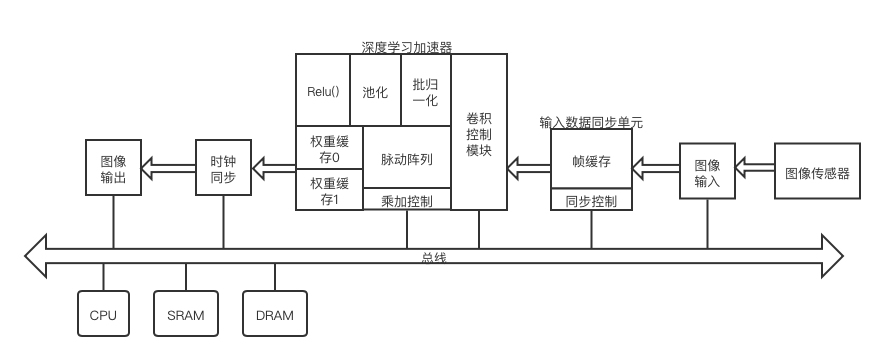
\includegraphics[width=15cm,height=6cm]{figures/top_arch.png}
    \caption{总体架构图}
    \label{fig:top_arch}
\end{figure}
%TODO 各个模块的简述
这里的视频数据格式为RGB888。
因此,我们可以轻松将其转化为深度学习加速器模块需要的输入数据尺寸224x224x3个像素点。




\section{数据通路中的模块}
图像数据通路的设计是本课题的核心部分。
CIS芯片的基本需求就是将光学图像转换成电信号,再将电信号经过模拟信号转换为数字信号。
在CIS芯片将数据转换为数字信号后,它还会将数字信号进行处理,输出用户需求的图像信息。
这个信号从前向后传输并转换的逻辑像一条通道,因此称之为图像数据通路。

本课题要做的就是在CIS芯片进行数字信号处理时,增加硬件加速的深度学习神经网络推理运算。
本章将分别阐明数据流的输入,数据的运算,数据流的输出三个部分的所有模块设计原理。
其中,各小节会着重描述数据流的组件间逻辑关系,以及各个模块控制流的状态机和执行逻辑。

\paragraph{模块需求}

一般的,在芯片中CPU用于执行固件的程序。
这些软件一般用于初始化设备,或者与主机通信。
图像数据的处理过程是由数据通路中的每个模块完成的。
这个小节将分析每个模块的功能,以及模块间的数据流和控制流关系。
首先,我们可以分解需求并得到以下列出的需求点:
\begin{enumerate}
    \item 数据通路中的基本模块
    \item 脉动阵列的设计
    \item ResNet18在脉动阵列上的实现
\end{enumerate}    

\subparagraph{数据通路}
数据通路的基本功能就是数据的输入、数据的处理和数据的输出。
对于深度学习神经网络加速器,我们需要设计一个配合加速器工作的数据信号输入模块。
这个模块需要根据后文描述的加速器的行为,将视频数据流中的数据按照加速器所需的数据宽度、数据格式和频率放置到加速器的输入缓冲中。
神经网络加速器就是整个数据通路中用于深度学习神经网络运算的模块。

\subparagraph{脉动阵列}
在脉动阵列中,需要设计每个处理单元的逻辑和工作行为。
在实现神经网络算法时,需要分解出所有使用到的运算符,并分析哪些可以通过脉动阵列的乘加运算矩阵加速。


\subsection{模块设计}
图像数据通路的整体设计如图所示\ref{fig:image_datapath},在整个图像数据通路中有三个不同的时钟域。
\begin{figure}[htbp]
    \centering
    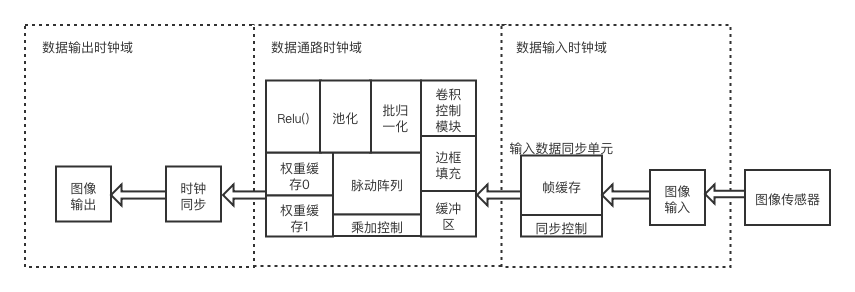
\includegraphics[width=15cm,height=6cm]{figures/image_datapath.png}
    \caption{图像数据通路架构图}
    \label{fig:image_datapath}
\end{figure}
区分这三个时钟域的目的是支持3个不同的时钟频率。
它们分别是图像传感器的输入数据信号的时钟、深度学习加速器的运行时钟和特征图的输出数据信号的时钟。
在这个数据通路中,最重要的模块就是深度学习运算加速器模块。


\subsection{数据流的输入}
% TODO 
%   数据流的输入将由IDA(Input Data Adapter)模块处理。这个模块的主要作用是将Sensor输出的数据放到一个缓存区。
%   并将视频数据流的plck同步到数据流的时钟域。

这里假设从图像传感器输出的图像数据为224x224像素尺寸的图像。
视频数据流的输入需要参考流式设备的特性,合理的缓存大小和同步的时机是关键点。
对于卷积运算,缓存的行数大小应该大于等于卷积核的行数和列数之间的较大值。
例如,卷积核的尺寸为3x3时,缓存至少要保存3行数据。
如果,每帧图像的尺寸为224x224个像素点。
由RGB三个通道组成的每一帧都拆分成三个224x224x8比特流。
那么需要给一个通道的一帧数据缓存的大小需要大于等于672个字节。







\begin{figure}[htbp]
    \centering
    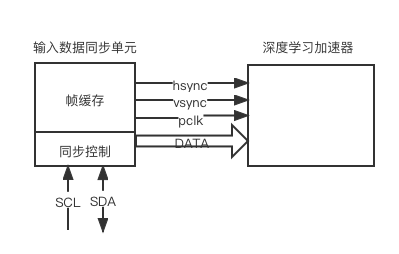
\includegraphics[width=12cm,height=8cm]{figures/input_data_adapter.png}
    \caption{输入数据同步单元架构图}
    \label{fig:input_data_adapter}
\end{figure}

如图\ref{fig:input_data_adapter}是数据输入同步单元与深度学习加速器之间的连线设计。
hsync用于行同步信号。
vsync用于帧同步信号。
pclk是像素时钟信号。
data是并行的图像数据,这里设定为8bit带宽。
SCL和SDA是用来读写模块寄存器的I2C接口的时钟信号和数据信号。


\subsection{数据流中的运算}
% TODO
% 在数据流中实时运算图像识别的算法
深度学习运算加速器是专用于进行深度学习运算的硬件加速模块。
它的作用是在数据通路中实时地进行图像识别的运算。
此设计选择了ResNet18作为实现的网络算法。
运算的模块将通过帧同步信号和行同步信号等机制来处理缓存的数据。
在实际应用时,将用于图像识别的人工智能处理器在物理位置上比较靠近图像来源(CMOS传感器),这样就避免了图像数据需要SRAM/DRAM的存储。
同时,还可以利用图像数据流的流水线特性,设计减小输入缓冲的图像输入模块。
依靠图像数据信号中的行同步信号和帧同步信号,来同步向数据通道后方的脉动阵列输送数据,那么就不需要缓冲多帧或者一个完整帧的数据。
另外,由于一般的CNN算法是共享权重的。这样权重的数量就不大,可以完整存放在片上SRAM中,从而使得读取权重的操作也能避免访问DRAM。
在设计权重缓冲区时,我们采用了多路缓冲的思想。将划分多个bank缓冲区,来分别缓冲不同卷积层的权重。
这样的话,权重缓冲区可以在脉动阵列工作时,加载后一层的权重到缓冲区中。
在需要进行下一层的运算时,脉动阵列就可以直接从SRAM的缓冲区中读取权重,而不是DRAM。
这样处理后,整个系统将大幅降低功耗。
% 单独画图解释一下权重缓冲区
% 单独画图解释一下行同步信号控制数据输入

整个深度学习加速器模块有2个缓存分别用于存储权重、输入数据。
核心的运算模块是由最小运算单元组成的脉动阵列。
普通的运算阵列受限于其规模。它的规模越大,需要的传输布线长度约长,传输时间越久,因此频率也无法做到很高。
这样的话,它的运算性能就会受到规模大小的限制。



\subsection{图像数据通路}
图像数据通路的需求是深度学习加速器的基础。
CIS芯片的作用,就是将图像传感器接收到的信号,转为数字信号后传输给后端。
芯片上图像数字信号所经过的所有模块连接起来就像是一条单向的通道。
一般的,我们称这些模块所组成的通道为图像数据通路。
图像数据通路一般由输入、数据处理和输出三个部分组成。
通常地,这三个部分也具有各自不同的时钟域。

%TODO 架构图展示
\begin{figure}[htbp]
    \centering
    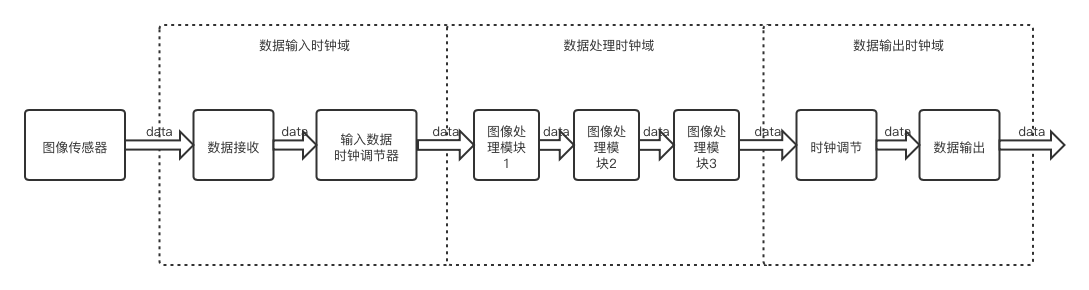
\includegraphics[width=15cm,height=5cm]{figures/datapath.png}
    \caption{图像信号处理的数据流图}
    \label{fig:datapath}
\end{figure}

%TODO 这里先描述以下datapath,包括DI、DP、DO三个时钟域。
如图\ref{fig:datapath}所示,图像处理部件的前后分别需要设置两个不同的时钟域用于输入和输出图像数据的信号。
因此,我们在设计CIS的数据通路中的深度学习运算模块时,也需要做相同的设计。
将输入模块的图像数据信号按一定的顺序排列好,按照脉动阵列的特性以一定的方式依次输入到阵列中。


在输入时钟域中,RX模块接收从CMOS传感器输出的数据。
由一个缓冲区暂存数据,经过时钟同步和一些预处理后向后面的数据处理时钟域输出数据。
在数据处理的时钟域中,深度学习运算模块将进行推理操作。
在输出时钟域中,FT(fix timing)模块将调整输出的时钟频率.TX模块负责以指定格式输出图像数据。  


\section{存储器的选择}
在设计嵌入式的深度学习加速器时,无论是系统级使用的存储或者是模块中的缓冲,都要选择合适的存储介质。
设计过程中要为不同模块设计所需的存储器或缓存。
存储器和缓存的设计直接影响了整个加速器模块或者深度学习运算芯片的运算能力。



